\documentclass[border=10pt]{standalone}
\usepackage{tikz}

\begin{document}
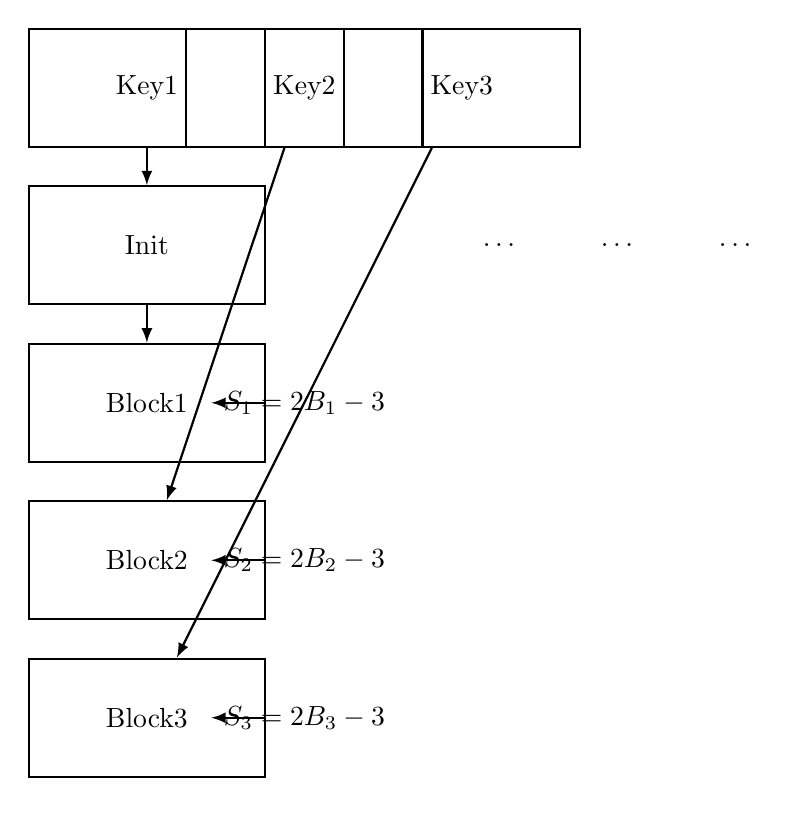
\begin{tikzpicture}[node distance=2cm, thick, main node/.style={rectangle, draw, minimum width=3cm, minimum height=1.5cm}]

    % Nodes for keys and blocks
    \node (key1) [main node] {Key1};
    \node (init) [main node, below of=key1] {Init};
    \node (block1) [main node, below of=init] {Block1};
    \node (s1) [circle, right of=block1] {$S_1 = 2B_1 - 3$};

    \draw [-latex] (key1) -- (init);
    \draw [-latex] (init) -- (block1);
    \draw [-latex] (block1) -- (s1);

    % Second set
    \node (key2) [main node, right of=key1] {Key2};
    \node (block2) [main node, below of=block1] {Block2};
    \node (s2) [circle, right of=block2] {$S_2 = 2B_2 - 3$};

    \draw [-latex] (key2) -- (block2);
    \draw [-latex] (block2) -- (s2);

    % Third set
    \node (key3) [main node, right of=key2] {Key3};
    \node (block3) [main node, below of=block2] {Block3};
    \node (s3) [circle, right of=block3] {$S_3 = 2B_3 - 3$};

    \draw [-latex] (key3) -- (block3);
    \draw [-latex] (block3) -- (s3);

    % Ellipsis
    \node at (4.5, -2) {\dots};
    \node at (6, -2) {\dots};
    \node at (7.5, -2) {\dots};

\end{tikzpicture}
\end{document}